\documentclass{beamer}\usepackage[]{graphicx}\usepackage[]{xcolor}
% maxwidth is the original width if it is less than linewidth
% otherwise use linewidth (to make sure the graphics do not exceed the margin)
\makeatletter
\def\maxwidth{ %
  \ifdim\Gin@nat@width>\linewidth
    \linewidth
  \else
    \Gin@nat@width
  \fi
}
\makeatother

\definecolor{fgcolor}{rgb}{0.345, 0.345, 0.345}
\newcommand{\hlnum}[1]{\textcolor[rgb]{0.686,0.059,0.569}{#1}}%
\newcommand{\hlstr}[1]{\textcolor[rgb]{0.192,0.494,0.8}{#1}}%
\newcommand{\hlcom}[1]{\textcolor[rgb]{0.678,0.584,0.686}{\textit{#1}}}%
\newcommand{\hlopt}[1]{\textcolor[rgb]{0,0,0}{#1}}%
\newcommand{\hlstd}[1]{\textcolor[rgb]{0.345,0.345,0.345}{#1}}%
\newcommand{\hlkwa}[1]{\textcolor[rgb]{0.161,0.373,0.58}{\textbf{#1}}}%
\newcommand{\hlkwb}[1]{\textcolor[rgb]{0.69,0.353,0.396}{#1}}%
\newcommand{\hlkwc}[1]{\textcolor[rgb]{0.333,0.667,0.333}{#1}}%
\newcommand{\hlkwd}[1]{\textcolor[rgb]{0.737,0.353,0.396}{\textbf{#1}}}%
\let\hlipl\hlkwb

\usepackage{framed}
\makeatletter
\newenvironment{kframe}{%
 \def\at@end@of@kframe{}%
 \ifinner\ifhmode%
  \def\at@end@of@kframe{\end{minipage}}%
  \begin{minipage}{\columnwidth}%
 \fi\fi%
 \def\FrameCommand##1{\hskip\@totalleftmargin \hskip-\fboxsep
 \colorbox{shadecolor}{##1}\hskip-\fboxsep
     % There is no \\@totalrightmargin, so:
     \hskip-\linewidth \hskip-\@totalleftmargin \hskip\columnwidth}%
 \MakeFramed {\advance\hsize-\width
   \@totalleftmargin\z@ \linewidth\hsize
   \@setminipage}}%
 {\par\unskip\endMakeFramed%
 \at@end@of@kframe}
\makeatother

\definecolor{shadecolor}{rgb}{.97, .97, .97}
\definecolor{messagecolor}{rgb}{0, 0, 0}
\definecolor{warningcolor}{rgb}{1, 0, 1}
\definecolor{errorcolor}{rgb}{1, 0, 0}
\newenvironment{knitrout}{}{} % an empty environment to be redefined in TeX

\usepackage{alltt}
\usepackage{graphicx}
\usepackage{graphicx}
\usepackage{verbatim}
\usepackage{etoolbox}
\usepackage{everysel}
% \usepackage{enumitem}

%% This package allows text highlighting
\usepackage{soul}

%% This sets the theme of the presentation which controls
%% the formatting of the slides
\usetheme{Boadilla}

%% Turn off the navigation symbols
\setbeamertemplate{navigation symbols}{} 

%% Change the default itemize [ball]s to [circle]s
\setbeamertemplate{itemize items}[circle]

%% Change the default enumerate [ball]s to plain text
\setbeamertemplate{enumerate items}[default]

%% Load the enumitem package and ensure it works nicely with beamer
% \setitemize{label=\usebeamerfont*{itemize item}
%   \usebeamercolor[fg]{itemize item}
%   \usebeamertemplate{itemize item}}
% \setenumerate{label=\usebeamerfont*{enumerate item}
%   \usebeamercolor[fg]{enumerate item}
%   \usebeamertemplate{enumerate item}}

%% Set the author block so STATS 201/8 appears on every
\author{STATS 201/8}

%% Clear the date block
\date{}


\setbeamercolor{title}{bg=blue!40}
\setbeamerfont{title}{size=\LARGE,series=\bfseries}

%%Sectioning commands
\setbeamercolor{section title}{bg=blue!20}
\setbeamerfont{section title}{size=\large}

\setbeamertemplate{section page}{%
    \begingroup
        \begin{beamercolorbox}[sep=10pt,center,rounded=true,shadow=true]{section title}
        \usebeamerfont{section title}Section~\thechapter.\thesection \newline \insertsection\par
        \end{beamercolorbox}
		\vfill
    \endgroup
}

\newcommand{\BeginSection}[1]{\section{#1} \frame{\sectionpage}}
%\AtBeginSection[]{%
%    \begin{frame}
%        \sectionpage
%    \end{frame}
%}


%% This makes all equations blue
\AtBeginEnvironment{equation*}{\color{blue}}
\AtBeginEnvironment{align*}{\color{blue}}
\everymath{\color{blue}}

%% This puts a 0 point space between paragraphs, means we don't need to use vspace, or list environments if 
%% we don't want to
\setlength{\parskip}{0pt}


%% Russell: removes spaces after R input/output?
\setlength{\topsep}{0.5mm}

%% David: In addition to Russel's command to remove spaces after R input/output, these commands remove the space between R input/output.
%% Stackoverflow link: https://stackoverflow.com/questions/35734525/reduce-space-between-code-chunks-and-code-output-in-rmarkdown-beamer-presentatio
%% \setlength{\OuterFrameSep}{-2pt}
\makeatletter
\preto{\@verbatim}{\topsep=-1pt \partopsep=-1pt }
\makeatother

%% Some useful colors
\definecolor{darkgreen}{rgb}{0.176,0.486,0.031}
\definecolor{redbrown}{HTML}{950605}
\definecolor{darkred}{HTML}{d80605}


%% nice little macro for changing the font of R code
\newcommand{\rcode}[1]{\protect{\color{darkgreen}\texttt{#1}}}

%% macro for bold blue italics
\newcommand{\blueBoldEmph}[1]{{\color{blue}\textbf{\emph{#1}}}}

% ~iid macro
\newcommand{\iid }{\stackrel{iid}{\sim}}

%% Macro for t-test amd P-value
\newcommand{\ttest}{\emph{t}-test}
\newcommand{\pval}{\emph{P}-value}

%% Statistics operators 
\DeclareMathOperator{\Bias}{Bias}
\DeclareMathOperator{\Cov}{Cov}
\DeclareMathOperator*{\Cor}{Cor}
\DeclareMathOperator{\E}{E}
\DeclareMathOperator{\MSE}{MSE}
\DeclareMathOperator{\Odds}{Odds}
\DeclareMathOperator{\OR}{OR}
\DeclareMathOperator{\PMSE}{PMSE}
\DeclareMathOperator{\sd}{sd}
\DeclareMathOperator{\se}{se}
\DeclareMathOperator*{\Var}{Var}
\DeclareMathOperator{\logit}{logit}

%% Should see if can make this a mathop
\newcommand{\comb}[2]{\mbox{$\big(_{#2}^{#1}\big)$}}



\IfFileExists{upquote.sty}{\usepackage{upquote}}{}
\begin{document}
\newcommand{\thechapter}{6}



\title{Chapter 6: \\ Multiplicative linear models}
\institute{University of Auckland}

\begin{frame}
\titlepage
\end{frame}


\begin{frame}[t]
\frametitle{Learning Outcomes}
In this chapter you will learn about:
\begin{center}
\vspace{16pt}
\begin{minipage}{0.9\textwidth}
  \begin{itemize}
  \item Mean versus median -- which to use?
  \item Transforming the response variable using the log function
  \item Multiplicative models
  \item Why inference is about the median (not the mean)
  \item A multiplicative simple linear regression example
  \item A multiplicative two-sample t-test example
  \item Relevant \rcode{R}-code.
  \end{itemize}
\end{minipage}
\end{center}
\end{frame}


%%%%%%%%%%%%%%%%%%%%%%%%%%%%%%%%%%%%%%%%%%%%%%%%%%%%%%%%%%%%%%%%%%%%%%%%%%%%%%%%%%%%%%%%%%%
\BeginSection{Mean versus median -- which to use?}
%%%%%%%%%%%%%%%%%%%%%%%%%%%%%%%%%%%%%%%%%%%%%%%%%%%%%%%%%%%%%%%%%%%%%%%%%%%%%%%%%%%%%%%%%%%


\begin{frame}[t]
\frametitle{Auckland house prices}
In early 2021 one of the STATS 20x lecturers was looking to buy a house in a working-class suburb of Auckland, about 15 minutes by train to downtown.\footnote{Auckland house prices are very high by international standards.}
\medskip

The lecturer downloaded 94 recent sales prices for the suburb, and put the prices (\$1000's) in a text file called \rcode{AkldHousePrices.txt}. The lecturer just wants to know the typical house price in the suburb -- there are no explanatory variables.
\bigskip

It sounds like an easy analysis. We just need to fit a null model. Let's take a look...
\end{frame}



\begin{frame}[fragile]
\frametitle{Auckland house prices\ldots}
\framesubtitle{Inspect the data}
\begin{knitrout}\scriptsize
\definecolor{shadecolor}{rgb}{0.969, 0.969, 0.969}\color{fgcolor}\begin{kframe}
\begin{alltt}
\hlstd{> }\hlstd{Houses.df}\hlkwb{=}\hlkwd{read.table}\hlstd{(}\hlstr{"Data/AkldHousePrices.txt"}\hlstd{,}\hlkwc{header}\hlstd{=T)}
\hlstd{> }\hlkwd{hist}\hlstd{(Houses.df}\hlopt{$}\hlstd{price,} \hlkwc{breaks}\hlstd{=}\hlnum{20}\hlstd{,}\hlkwc{main}\hlstd{=}\hlstr{""}\hlstd{,}\hlkwc{xlab}\hlstd{=}\hlstr{"Price ($1000)"}\hlstd{)}
\hlstd{> }\hlkwd{abline}\hlstd{(}\hlkwc{v} \hlstd{=} \hlkwd{c}\hlstd{(}\hlkwd{mean}\hlstd{(Houses.df}\hlopt{$}\hlstd{price),} \hlkwd{median}\hlstd{(Houses.df}\hlopt{$}\hlstd{price)),}
\hlstd{+ }       \hlkwc{col} \hlstd{=} \hlkwd{c}\hlstd{(}\hlstr{"blue"}\hlstd{,} \hlstr{"green"}\hlstd{),} \hlkwc{lwd} \hlstd{=} \hlnum{2}\hlstd{)}
\end{alltt}
\end{kframe}
\end{knitrout}



\begin{figure}
  \centering
  \includegraphics{figure/RC-H06-002}
\end{figure}

\end{frame}



\begin{frame}[fragile,t]
\frametitle{Auckland house prices\ldots}
\framesubtitle{Inspect the data...}
\begin{knitrout}\scriptsize
\definecolor{shadecolor}{rgb}{0.969, 0.969, 0.969}\color{fgcolor}\begin{kframe}
\begin{alltt}
\hlstd{> }\hlkwd{summary}\hlstd{(Houses.df}\hlopt{$}\hlstd{price)}
\end{alltt}
\begin{verbatim}
   Min. 1st Qu.  Median    Mean 3rd Qu.    Max. 
  450.0   832.5  1130.0  1310.1  1597.5  3710.0 
\end{verbatim}
\end{kframe}
\end{knitrout}
\bigskip
Clearly, we are not dealing with data that come from a normal distribution.  See how the (sample) median is markedly lower than the (sample) mean. \\
\bigskip 
This type of right-skew distribution is very common when it comes to things involving money
(\$\$\$), resources, growth, salary, age, advantage and energy, to name but a few.
\bigskip

We can still make inference using a linear model for the expected house price because we can apply the \textbf{CLT} since we have a largish number of observations ($n=94$).
Alternatively, we can use the bootstrap since it does not require the assumption of normality.
\end{frame}




\begin{frame}[fragile]
\frametitle{Auckland house prices\ldots}
\framesubtitle{Inference about the mean}
Here is histogram of 10,000 bootstrap sample means from resampling the house price data.



\begin{figure}
  \centering
  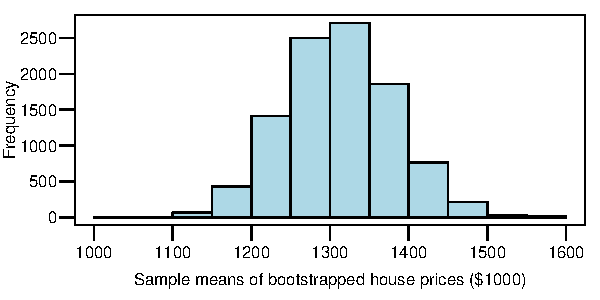
\includegraphics{figure/RC-H06-004}
\end{figure}

The approximate normality ot the bootstrapped sample means shows that the sample mean has 
an approximate normal distribution.
\end{frame}



\begin{frame}[fragile]
\frametitle{Auckland house prices\ldots}
\framesubtitle{Inference  about the mean\ldots}

Here is the bootstrap 95\% CI for the expected price, along with output from the null model.

\begin{knitrout}\scriptsize
\definecolor{shadecolor}{rgb}{0.969, 0.969, 0.969}\color{fgcolor}\begin{kframe}
\begin{alltt}
\hlstd{> }\hlkwd{quantile}\hlstd{(bootstrappedMeanPrices,} \hlkwd{c}\hlstd{(}\hlnum{.025}\hlstd{,} \hlnum{.975}\hlstd{))}
\end{alltt}
\begin{verbatim}
    2.5%    97.5% 
1181.168 1452.875 
\end{verbatim}
\end{kframe}
\end{knitrout}

\begin{knitrout}\scriptsize
\definecolor{shadecolor}{rgb}{0.969, 0.969, 0.969}\color{fgcolor}\begin{kframe}
\begin{alltt}
\hlstd{> }\hlstd{HousesNull.fit}\hlkwb{=}\hlkwd{lm}\hlstd{(price}\hlopt{~}\hlnum{1}\hlstd{,} \hlkwc{data}\hlstd{=Houses.df)}
\hlstd{> }\hlkwd{summary}\hlstd{(HousesNull.fit)}
\end{alltt}
\end{kframe}
\end{knitrout}

\begin{knitrout}\scriptsize
\definecolor{shadecolor}{rgb}{0.969, 0.969, 0.969}\color{fgcolor}\begin{kframe}
\begin{verbatim}
Coefficients:
            Estimate Std. Error t value Pr(>|t|)    
(Intercept)   1310.1       70.1   18.69   <2e-16 ***
---
Residual standard error: 679.7 on 93 degrees of freedom
\end{verbatim}
\end{kframe}
\end{knitrout}

\begin{knitrout}\scriptsize
\definecolor{shadecolor}{rgb}{0.969, 0.969, 0.969}\color{fgcolor}\begin{kframe}
\begin{alltt}
\hlstd{> }\hlkwd{confint}\hlstd{(HousesNull.fit)}
\end{alltt}
\begin{verbatim}
               2.5 %   97.5 %
(Intercept) 1170.899 1449.313
\end{verbatim}
\end{kframe}
\end{knitrout}

Here we see that, to within less than NZ\$10\,000,  the bootstrap CI and the model CI are the same. This is confirmation that the \textbf{CLT}  works.
\end{frame}


\begin{frame}[fragile]
\frametitle{Auckland house prices\ldots}
\framesubtitle{Inference  about the mean\ldots}
So we can safely say that the mean (i.e., expected) sale price for the entire suburb is somewhere between, say, NZ\$1.17 million to NZ\$1.45 million.
However, the gross non-normality of the data prevents us from making prediction intervals for house prices. 

\medskip Moreover, the estimated mean price of NZ\$1.31 million is somewhat misleading.\footnote{It is also not statistically robust since it is very sensitive to the number of expensive ($\geq$ \$3 million, say) houses sold}
Our house-hunting lecturer just wants a typical house, about midway in affordability at most. It would make more sense to estimate the {\bf median} house price, since our lecturer will then know that half of the houses going on the property market will sell for less than that price.
\medskip

In general, for highly skewed data the median is usually a better measure of `typical' value than the mean.
\end{frame}



\begin{frame}[fragile]
\frametitle{Auckland house prices\ldots}
\framesubtitle{Inference about the median}

To estimate the median sale price of the entire suburb the natural estimate is the median of our sample:
\begin{knitrout}\scriptsize
\definecolor{shadecolor}{rgb}{0.969, 0.969, 0.969}\color{fgcolor}\begin{kframe}
\begin{alltt}
\hlstd{> }\hlkwd{median}\hlstd{(Houses.df}\hlopt{$}\hlstd{price)}
\end{alltt}
\begin{verbatim}
[1] 1130
\end{verbatim}
\end{kframe}
\end{knitrout}
and we can use a bootstrap to get a 95\% CI for the suburb median
\begin{knitrout}\scriptsize
\definecolor{shadecolor}{rgb}{0.969, 0.969, 0.969}\color{fgcolor}\begin{kframe}
\begin{alltt}
\hlstd{> }\hlkwd{quantile}\hlstd{(bootstrappedMedianPrices,} \hlkwd{c}\hlstd{(}\hlnum{.025}\hlstd{,} \hlnum{.975}\hlstd{))}
\end{alltt}
\begin{verbatim}
 2.5% 97.5% 
 1040  1320 
\end{verbatim}
\end{kframe}
\end{knitrout}
so we can say that the median sale price for the entire suburb is somewhere between,
say, NZ\$1.04 million to NZ\$1.32 million.
\bigskip

The 95\% CI for the median comes as something of a relief to our house-hunting lecturer. It is much more reasonable than the \$1.17 to \$1.45 million CI for the mean which was markedly higher due to the data being so right-skewed. 
\end{frame}


\begin{frame}[fragile]
\frametitle{Inference about the median}

In the above house price example we are working with iid data, 
so it is natural to use the sample median to estimate the population median.
\bigskip \bigskip

We'll see in the next section that the linear model framework can also be used to make
inference about the median provided that the logged response variable is approximately normally distributed.
This approach has the advantage that it can also be applied to more general situations where we have explanatory variables that may be associated with the response variable. 
\medskip

We'll also see that fitting linear models to logged response data results in the effects of explanatory variables acting multiplicatively on medians.

\end{frame}


%%%%%%%%%%%%%%%%%%%%%%%%%%%%%%%%%%%%%%%%%%%%%%%%%%%%%%%%%%%%%%%%%%%%%%%%%%%%%%%%%%%%%%%%%%%
\BeginSection{Transforming the response variable using the log function}
%%%%%%%%%%%%%%%%%%%%%%%%%%%%%%%%%%%%%%%%%%%%%%%%%%%%%%%%%%%%%%%%%%%%%%%%%%%%%%%%%%%%%%%%%%%

\begin{frame}[fragile]
\frametitle{Auckland house prices\ldots}
\framesubtitle{Transforming the data}
Let's consider making a transformation of the prices. In particular, the log transformation.
Here is the histogram of \rcode{log(price)}.



\begin{figure}
  \centering
  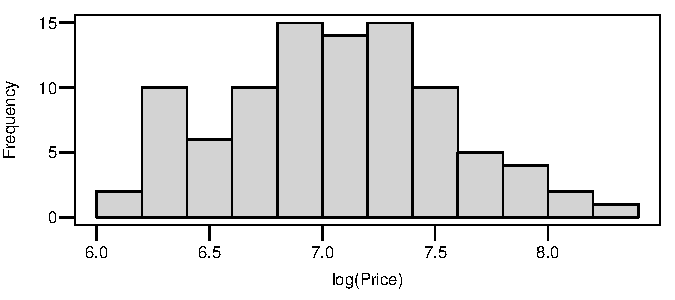
\includegraphics{figure/RC-H06-010}
\end{figure}

This looks reasonably close to normal, so if we fit a linear model to these data then all inferences will be valid.
\end{frame}



\begin{frame}[fragile]
\frametitle{Auckland house prices\ldots}
\framesubtitle{Null model fitted to logged house price data}
\begin{knitrout}\scriptsize
\definecolor{shadecolor}{rgb}{0.969, 0.969, 0.969}\color{fgcolor}\begin{kframe}
\begin{alltt}
\hlstd{> }\hlstd{LoggedPriceNull.fit}\hlkwb{=}\hlkwd{lm}\hlstd{(}\hlkwd{log}\hlstd{(price)}\hlopt{~}\hlnum{1}\hlstd{,} \hlkwc{data}\hlstd{=Houses.df)}
\hlstd{> }\hlkwd{coef}\hlstd{(}\hlkwd{summary}\hlstd{(LoggedPriceNull.fit))}
\end{alltt}
\begin{verbatim}
            Estimate Std. Error  t value      Pr(>|t|)
(Intercept) 7.060405 0.04974049 141.9448 1.628721e-110
\end{verbatim}
\end{kframe}
\end{knitrout}

\begin{knitrout}\scriptsize
\definecolor{shadecolor}{rgb}{0.969, 0.969, 0.969}\color{fgcolor}\begin{kframe}
\begin{alltt}
\hlstd{> }\hlkwd{confint}\hlstd{(LoggedPriceNull.fit)}
\end{alltt}
\begin{verbatim}
              2.5 %  97.5 %
(Intercept) 6.96163 7.15918
\end{verbatim}
\end{kframe}
\end{knitrout}

Well that is interesting, but logged house prices don't mean much to anyone who is hoping to buy a house. The inference needs to be back-transformed to NZ\$. 

Since we've used the log transformation, the back-transformation is the exponential function \rcode{exp()}.

\begin{knitrout}\scriptsize
\definecolor{shadecolor}{rgb}{0.969, 0.969, 0.969}\color{fgcolor}\begin{kframe}
\begin{alltt}
\hlstd{> }\hlkwd{exp}\hlstd{(}\hlkwd{confint}\hlstd{(LoggedPriceNull.fit))}
\end{alltt}
\begin{verbatim}
               2.5 %   97.5 %
(Intercept) 1055.353 1285.856
\end{verbatim}
\end{kframe}
\end{knitrout}

\end{frame}



\begin{frame}[fragile]
\frametitle{Auckland house prices\ldots}
\framesubtitle{The effect of transforming}
The above confidence interval is quite different from the one we calculated for the mean house price of the suburb. The reason for this is because the above CI is for the {\bf median} house price. 
\medskip

To see why this is, let's take a look at what happens when we transform summary statistics using the \rcode{log()} and \rcode{exp()} functions: 
\medskip

Summaries of price:
\begin{knitrout}\scriptsize
\definecolor{shadecolor}{rgb}{0.969, 0.969, 0.969}\color{fgcolor}\begin{kframe}
\begin{alltt}
\hlstd{> }\hlkwd{summary}\hlstd{(Houses.df}\hlopt{$}\hlstd{price);}
\end{alltt}
\begin{verbatim}
   Min. 1st Qu.  Median    Mean 3rd Qu.    Max. 
  450.0   832.5  1130.0  1310.1  1597.5  3710.0 
\end{verbatim}
\end{kframe}
\end{knitrout}
Summaries of log(price):
\begin{knitrout}\scriptsize
\definecolor{shadecolor}{rgb}{0.969, 0.969, 0.969}\color{fgcolor}\begin{kframe}
\begin{alltt}
\hlstd{> }\hlkwd{summary}\hlstd{(}\hlkwd{log}\hlstd{(Houses.df}\hlopt{$}\hlstd{price))}
\end{alltt}
\begin{verbatim}
   Min. 1st Qu.  Median    Mean 3rd Qu.    Max. 
  6.109   6.724   7.030   7.060   7.376   8.219 
\end{verbatim}
\end{kframe}
\end{knitrout}
Back-transformed summaries of log(price):
\begin{knitrout}\scriptsize
\definecolor{shadecolor}{rgb}{0.969, 0.969, 0.969}\color{fgcolor}\begin{kframe}
\begin{alltt}
\hlstd{> }\hlkwd{exp}\hlstd{(}\hlkwd{summary}\hlstd{(}\hlkwd{log}\hlstd{(Houses.df}\hlopt{$}\hlstd{price)))}
\end{alltt}
\begin{verbatim}
   Min. 1st Qu.  Median    Mean 3rd Qu.    Max. 
  450.0   832.5  1130.0  1164.9  1597.0  3710.0 
\end{verbatim}
\end{kframe}
\end{knitrout}

%As a result the summary values that just depend on the ordering of the values (e.g., minimum, %lower quartile, median, upper quartile, maximum) statistics are not affected.\footnote{The %order statistics for a sample are those that just depend on the order of the observations.} 
\end{frame}



\begin{frame}[fragile]
\frametitle{Auckland house prices\ldots}
\framesubtitle{The effect of transforming\ldots}

Note that the sample mean changed after transforming then back-transforming, but the other summary values did not. This is because transforming and back-transforming does not change the order of the data -- the smallest value will still be the smallest value, the middle value will still be the middle value.

\end{frame}



\begin{frame}[fragile]
\frametitle{Auckland house prices\ldots}
\framesubtitle{Why inference is about the population median}
If the logged response variable is normally distributed, then on the log scale its population mean and median are exactly the same number.\footnote{The sample mean and median may differ a little, as we saw with the logged house prices} 
In that case, a 95\% confidence interval for the population mean of the logged response variable is also a 95\% CI for the population median of the logged response variable.
\medskip

Since the median is unaffected by transforming and back-transforming, it follows that back-transforming the above 95\% confidence interval will give a 95\% confidence interval for the population median on the original scale. However, it will not be a 95\% confidence interval for the population mean.
\medskip

We now have a recipe for calculating a confidence interval for the {\bf median} -- fit a linear model to the log-transformed data, calculate a 95\% confidence interval for the {\bf mean} (and hence {\bf median}), and back transform.
\end{frame}


\begin{frame}[fragile]
\frametitle{Auckland house prices\ldots}
\framesubtitle{Inference about the median}
Our back-transformed estimate ($\exp(\hat{\beta}_0)$) 
and 95\% CI for the median suburb sale price are
\begin{knitrout}\scriptsize
\definecolor{shadecolor}{rgb}{0.969, 0.969, 0.969}\color{fgcolor}\begin{kframe}
\begin{alltt}
\hlstd{> }\hlkwd{exp}\hlstd{(}\hlkwd{coef}\hlstd{(LoggedPriceNull.fit))}
\end{alltt}
\begin{verbatim}
(Intercept) 
   1164.917 
\end{verbatim}
\begin{alltt}
\hlstd{> }\hlkwd{exp}\hlstd{(}\hlkwd{confint}\hlstd{(LoggedPriceNull.fit))}
\end{alltt}
\begin{verbatim}
               2.5 %   97.5 %
(Intercept) 1055.353 1285.856
\end{verbatim}
\end{kframe}
\end{knitrout}

So we can say we are reasonably sure (95\% confident) that the median house price is somewhere between NZ\$1.06 and NZ\$1.29 million.
\bigskip

These values differ a little from the sample median (NZ\$1130) and the 95\% bootstrap CI
of NZ\$1040 to NZ\$1320 we saw in the previous section. 
This is because the machinery being used is different.

\bigskip

 
\bigskip

\end{frame}



\begin{frame}
\frametitle{Auckland house prices\ldots}
\framesubtitle{Inference for the house price data}

Here is the confidence interval for the mean suburb price with the sample mean shown in blue.


\begin{figure}
  \centering
  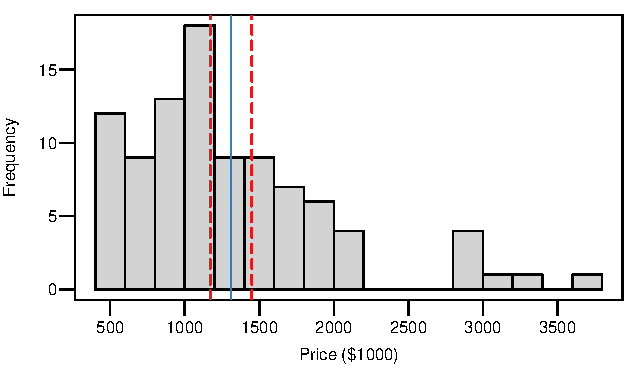
\includegraphics{figure/RC-H06-017}
\end{figure}

\end{frame}


\begin{frame}
\frametitle{Auckland house prices\ldots}
\framesubtitle{Inference for the house price data\ldots}

Here is the confidence interval for the median suburb price with the estimate obtained from the linear model approach ($\exp(\hat{\beta}_0)$) shown in green.


\begin{figure}
  \centering
  \includegraphics{figure/RC-H06-018}
\end{figure}

\end{frame}


\begin{frame}
\frametitle{Auckland house prices\ldots}
\framesubtitle{Inference for the house price data\ldots}

Here is the above plot with the sample mean and sample median shown as well.


\begin{figure}
  \centering
  \includegraphics{figure/RC-H06-019}
\end{figure}

\end{frame}


%%%%%%%%%%%%%%%%%%%%%%%%%%%%%%%%%%%%%%%%%%%%%%%%%%%%%%%%%%%%%%%%%%%%%%%%%%%%%%%%%%%%%%%%%%%
\BeginSection{The log function turns multiplicative effects in to additive effects}
%%%%%%%%%%%%%%%%%%%%%%%%%%%%%%%%%%%%%%%%%%%%%%%%%%%%%%%%%%%%%%%%%%%%%%%%%%%%%%%%%%%%%%%%%%%


\begin{frame}[fragile]
\frametitle{Why the log transformation?}
In the above house price example it would have been possible to use many other choices for our transformation of the prices. How did we know that the log-transformation would transform the data to be approximately normally distributed? We didn't! But, the log transformation has a very special property that makes it a very sensible choice.
{\bf The log transformation turns multiplicative effects in to additive effects.}
\medskip

In many situations, the response variable is subject to effects that act multiplicatively. E.g., would proximity to a train station act additively or multiplicatively on the price of a house?\footnote{In other words, does being close to the train station make a house worth, say, \$150,000 more, or 10\% more?} What about having a view or being beside the estuary?
\medskip

In such cases, taking the log of the response variable results in these effects acting additively on the log scale...and by virtue of the CLT, the consequence of a lot of effects adding together is approximate normality on the log scale.

\end{frame}

\begin{frame}[fragile]
\frametitle{Logarithm refresher}
\framesubtitle{Turning multiplication in to addition}
You have used logarithms before.
When you multiply $100$ by $100,000$ you add the zeroes to create $10,000,000$.
That is, two $0$s + five $0$s = seven $0$s = $10,000,000$. 
More formally:
\[ 100\times 100,000 =10^{2}\times 10^{5}=10^{2+5}=10^7=10,000,000 \] \\[-5mm]

Using base 10 (the number of fingers/toes we humans have) we can write $log_{10}({100})=log_{10}({10^2})=2$.
So , 
\begin{align*}
log_{10}(100\times 100,000)&=log_{10}(10^2\times 10^5) \\
                        &=log_{10}(10^{2+5})=2+5=7 \\
                        &=log_{10}(100)+log_{10}(100,000) \ .\\
\end{align*}
\vspace{-30pt}

So we see that the log of a product (i.e., multiplication) is the sum (i.e, addition) of the logs. 

\begin{columns}
\begin{column}{0.85\textwidth}
{\scriptsize In Springfield, they {\em should} work in base 8.
This means that``100'' in Springfield would correspond to our 64.}
\end{column}
\begin{column}{0.15\textwidth}

\includegraphics[width=0.6in]{BartSimpson.jpg}
\end{column}
\end{columns}
\end{frame}



\begin{frame}[fragile]
\frametitle{Logarithm refresher\ldots}
\frametitle{Why use base $e$?}

In the scientific world we use base $e$ logarithms\footnote{$e=\lim_{n\to\infty}(1+\frac{1}{n})^{n}= 2.718282\ldots$} ($\log_e$) which are referred to as natural logs\footnote{Some programming languages and books use $\ln$ for the $\log_e$ function.}. 
\bigskip

In \rcode{R} the \rcode{log} function is the natural logarithm. If you need to calculate the logarithm base 10, then you can use the \rcode{log10} function, or type \rcode{log(x, base = 10)}, where \rcode{x} is the value for which you are trying to calculate the logarithm.\\
\bigskip
In many situations, it does not matter which base you use as the laws of logarithms hold regardless of the base you use. That is,
\[
\log_b(x\times y)=\log_b(x)+\log_b(y)
\]
for any base $b>0$, and values $x,y>0$.
\end{frame}


\begin{frame}[fragile]
\frametitle{The inverse log function, $e^x$}
\framesubtitle{Turning addition in to multipication\ldots}

Because we use natural logs ($\log_e$), it follows that the inverse transformation (i.e., back transformation) is the exponential function. This is the \rcode{exp} function in {\rcode R}. 
\medskip

Exponentiating a sum is equivalent to multiplying the separate exponentials. 
That is,
\[ e^{x+y} = e^x \times e^y \]
For example:

\begin{knitrout}\scriptsize
\definecolor{shadecolor}{rgb}{0.969, 0.969, 0.969}\color{fgcolor}\begin{kframe}
\begin{alltt}
\hlstd{> }\hlkwd{exp}\hlstd{(}\hlnum{2}\hlstd{)}
\end{alltt}
\begin{verbatim}
[1] 7.389056
\end{verbatim}
\begin{alltt}
\hlstd{> }\hlkwd{exp}\hlstd{(}\hlnum{3}\hlstd{)}
\end{alltt}
\begin{verbatim}
[1] 20.08554
\end{verbatim}
\begin{alltt}
\hlstd{> }\hlkwd{exp}\hlstd{(}\hlnum{2}\hlopt{+}\hlnum{3}\hlstd{)}
\end{alltt}
\begin{verbatim}
[1] 148.4132
\end{verbatim}
\begin{alltt}
\hlstd{> }\hlkwd{exp}\hlstd{(}\hlnum{2}\hlstd{)}\hlopt{*}\hlkwd{exp}\hlstd{(}\hlnum{3}\hlstd{)}
\end{alltt}
\begin{verbatim}
[1] 148.4132
\end{verbatim}
\end{kframe}
\end{knitrout}
\end{frame}


%%%%%%%%%%%%%%%%%%%%%%%%%%%%%%%%%%%%%%%%%%%%%%%%%%%%%%%%%%%%%%%%%%%%%%%%%%%%%%%%%%%%%%%%%%%
\BeginSection{Example 1: Multiplicative simple linear regression model}
%%%%%%%%%%%%%%%%%%%%%%%%%%%%%%%%%%%%%%%%%%%%%%%%%%%%%%%%%%%%%%%%%%%%%%%%%%%%%%%%%%%%%%%%%%%


\begin{frame}[fragile]
\frametitle{Multiplicative model with numerical explanatory variable}
\framesubtitle{Mazda price data}
When we also have explanatory variables ($x$), using the log transformation (applied to the response variable $y$) changes the shape of the relationship between $x$ and $y$ from additive to multiplicative. This is because we use the exponential to back-transform our additive linear model fitted to $\log(y)$.
\bigskip

We demonstrate with a new example: \\
\medskip
The year of manufacturer and asking price of 123 Mazda cars were collected from the Melbourne Age newspaper in 1991. The variables measured were:
\bigskip

\begin{center}
\begin{tabular}{ll}
\rcode{price}& price of vehicle in Australian \$ \\
\rcode{year}&	year of manufacture ($1990 = 90$) \\
\end{tabular}
\end{center}
\bigskip

We will assume that these data are a random sample from the population.\footnote{What would the population be here?}
\end{frame}


\begin{frame}[fragile]
\frametitle{Multiplicative model with numerical explanatory variable}
\framesubtitle{Depreciation of Mazda cars}
Here we wish to understand how the cars lose value as they age. We have the year the car was manufactured so we can ascertain its age since these data were collected in 1991 (or '91). That is, \rcode{age=91-year}. \\
\bigskip
\textbf{Intuition:} What does common sense tell us about the shape of the relationship between car price and age? That is, what do we \emph{expect} to see?
\bigskip

\begin{itemize}
\item An additive decrease in price with age? 
\item A multiplicative decrease in price with age?
\end{itemize}
\end{frame}


\begin{frame}[fragile]
\frametitle{Multiplicative model with numerical explanatory variable}
\framesubtitle{Depreciation of Mazda cars\ldots}
\begin{knitrout}\scriptsize
\definecolor{shadecolor}{rgb}{0.969, 0.969, 0.969}\color{fgcolor}\begin{kframe}
\begin{alltt}
\hlstd{> }\hlstd{Mazda.df} \hlkwb{=} \hlkwd{read.table}\hlstd{(}\hlstr{"Data/mazda.txt"}\hlstd{,}\hlkwc{header}\hlstd{=T)}
\hlstd{> }\hlstd{Mazda.df}\hlopt{$}\hlstd{age} \hlkwb{=} \hlnum{91} \hlopt{-} \hlstd{Mazda.df}\hlopt{$}\hlstd{year} \hlcom{## Create the age variable}
\hlstd{> }\hlkwd{plot}\hlstd{(price}\hlopt{~}\hlstd{age,} \hlkwc{data} \hlstd{= Mazda.df,} \hlkwc{xlab} \hlstd{=} \hlstr{"Age"}\hlstd{,} \hlkwc{ylab} \hlstd{=} \hlstr{"Price (AUD)"}\hlstd{)}
\end{alltt}
\end{kframe}
\end{knitrout}



\begin{figure}
  \centering
  \includegraphics{figure/RC-H06-021}
\end{figure}

\end{frame}


\begin{frame}[fragile]
\frametitle{Multiplicative model with numerical explanatory variable}
\framesubtitle{Depreciation of Mazda cars\ldots}
Let us look at the two components we are interested in, trend and scatter. 



\begin{figure}
  \centering
  \includegraphics{figure/RC-H06-022}
\end{figure}

% Here we see increased scatter with higher prices and a non-linear
% relationship between age and price.
\end{frame}


\begin{frame}[fragile]
\frametitle{Multiplicative model with numerical explanatory variable}
\framesubtitle{Depreciation of Mazda cars: A na\"ive price vs age models}
The trend is decreasing (exponentially), along with decreasing scatter -- these are classic symptoms of an underlying multiplicative model. Assuming \textbf{EOV} would be na\"ive in this case. Let us be na\"ive and see where it takes us. Let us fit a a linear model and see what the residual plot tells us.

\end{frame}


\begin{frame}[fragile]
\frametitle{Multiplicative model with numerical explanatory variable}
\framesubtitle{Na\"ive price vs age models\ldots}

\begin{knitrout}\scriptsize
\definecolor{shadecolor}{rgb}{0.969, 0.969, 0.969}\color{fgcolor}\begin{kframe}
\begin{alltt}
\hlstd{> }\hlstd{PriceAge.fit}\hlkwb{=}\hlkwd{lm}\hlstd{(price}\hlopt{~}\hlstd{age,} \hlkwc{data}\hlstd{=Mazda.df)}
\hlstd{> }\hlkwd{plot}\hlstd{(PriceAge.fit,}\hlkwc{which}\hlstd{=}\hlnum{1}\hlstd{)}
\end{alltt}
\end{kframe}
\end{knitrout}



\begin{figure}
  \centering
  \includegraphics{figure/RC-H06-024}
\end{figure}

\end{frame}


\begin{frame}[fragile]
\frametitle{Multiplicative model with numerical explanatory variable}
\framesubtitle{Na\"ive price vs age models\ldots}
The decreasing non-linear trend and non-constant scatter has become even more apparent.
Note: the higher fitted values on the horizontal axis are associated with newer cars. 
Let us be slightly less na\"ive and deal with the trend by fitting a quadratic term.

\end{frame}


\begin{frame}[fragile]
\frametitle{Multiplicative model with numerical explanatory variable}
\framesubtitle{Na\"ive price vs age models\ldots}
\begin{knitrout}\scriptsize
\definecolor{shadecolor}{rgb}{0.969, 0.969, 0.969}\color{fgcolor}\begin{kframe}
\begin{alltt}
\hlstd{> }\hlstd{PriceAge.fit2}\hlkwb{=}\hlkwd{lm}\hlstd{(price}\hlopt{~}\hlstd{age}\hlopt{+}\hlkwd{I}\hlstd{(age}\hlopt{^}\hlnum{2}\hlstd{),} \hlkwc{data}\hlstd{=Mazda.df)}
\hlstd{> }\hlkwd{plot}\hlstd{(PriceAge.fit2,}\hlkwc{which}\hlstd{=}\hlnum{1}\hlstd{)}
\end{alltt}
\end{kframe}
\end{knitrout}



\begin{figure}
  \centering
  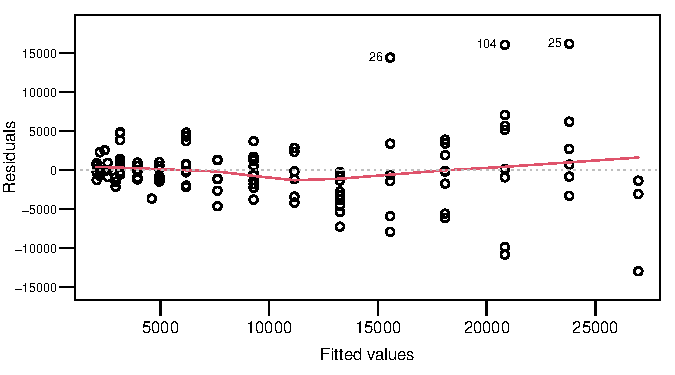
\includegraphics{figure/RC-H06-026}
\end{figure}

\end{frame}


\begin{frame}[fragile]
\frametitle{Multiplicative model with numerical explanatory variable}
\framesubtitle{Multiplicative price vs age model}
We have eliminated trend from these residuals but the \textbf{EOV} assumption is still violated.
Let us `tear up' this approach and take logs of price.



\begin{figure}
  \centering
  \includegraphics{figure/RC-H06-027}
\end{figure}

This is something we have seen before, is it not?
\end{frame}

\begin{frame}[fragile, t]
\frametitle{Multiplicative model with numerical explanatory variable}
\framesubtitle{Multiplicative price vs age model\ldots}
Let us fit the more appropriate multiplicative model.
\begin{knitrout}\scriptsize
\definecolor{shadecolor}{rgb}{0.969, 0.969, 0.969}\color{fgcolor}\begin{kframe}
\begin{alltt}
\hlstd{> }\hlstd{LogPriceAge.fit}\hlkwb{=}\hlkwd{lm}\hlstd{(}\hlkwd{log}\hlstd{(price)}\hlopt{~}\hlstd{age,} \hlkwc{data}\hlstd{=Mazda.df)}
\hlstd{> }\hlkwd{plot}\hlstd{(LogPriceAge.fit,}\hlkwc{which}\hlstd{=}\hlnum{1}\hlstd{)}
\end{alltt}
\end{kframe}
\end{knitrout}



\begin{figure}
  \centering
  \includegraphics{figure/RC-H06-029}
\end{figure}

\textbf{EOV} assumption is now satisfied. 

\end{frame}


\begin{frame}[fragile]
\frametitle{Multiplicative model with numerical explanatory variable}
\framesubtitle{Multiplicative price vsage model\ldots }
Check for normality of the residuals.
\begin{knitrout}\scriptsize
\definecolor{shadecolor}{rgb}{0.969, 0.969, 0.969}\color{fgcolor}\begin{kframe}
\begin{alltt}
\hlstd{> }\hlkwd{normcheck}\hlstd{(LogPriceAge.fit)}
\end{alltt}
\end{kframe}
\end{knitrout}



\begin{figure}
  \centering
  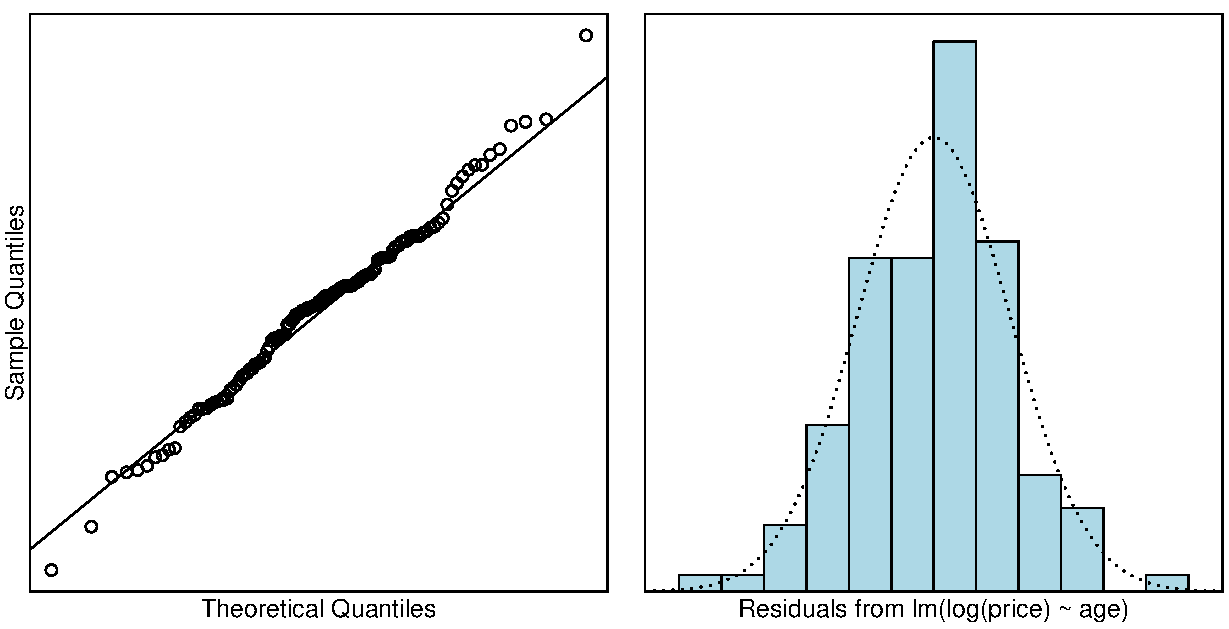
\includegraphics[scale=0.5]{figure/RC-H06-031}
\end{figure}

Normality assumption seems justified.
\end{frame}


\begin{frame}[fragile]
\frametitle{Multiplicative model with numerical explanatory variable}
\framesubtitle{Multiplicative price vs age model\ldots}
Check for unduly influential data points.
  
\begin{knitrout}\scriptsize
\definecolor{shadecolor}{rgb}{0.969, 0.969, 0.969}\color{fgcolor}\begin{kframe}
\begin{alltt}
\hlstd{> }\hlkwd{cooks20x}\hlstd{(LogPriceAge.fit)}
\end{alltt}
\end{kframe}
\end{knitrout}



\begin{figure}
  \centering
  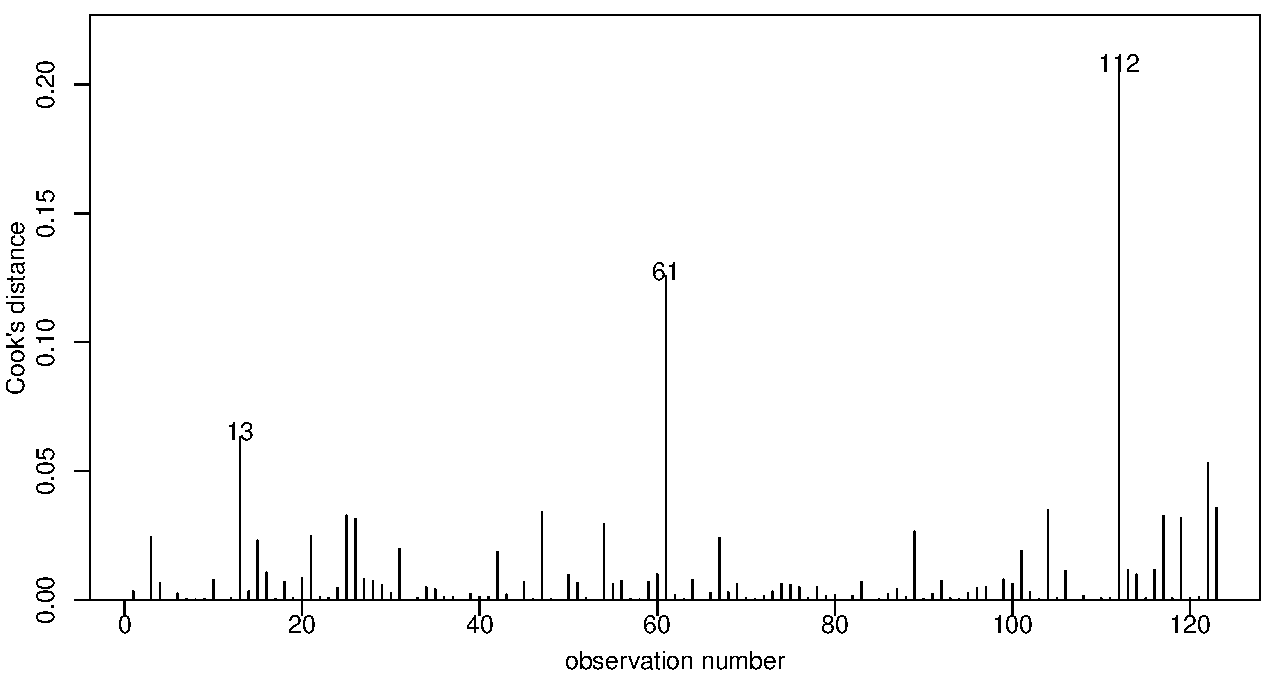
\includegraphics[scale=0.5]{figure/RC-H06-033}
\end{figure}

It looks fine.
\end{frame}


\begin{frame}[fragile]
\frametitle{Multiplicative model with numerical explanatory variable}
\framesubtitle{Multiplicative price vs age model\ldots}
Our assumptions are sound, so we can trust the resulting output.

\begin{knitrout}\scriptsize
\definecolor{shadecolor}{rgb}{0.969, 0.969, 0.969}\color{fgcolor}\begin{kframe}
\begin{alltt}
\hlstd{> }\hlkwd{summary}\hlstd{(LogPriceAge.fit)}
\end{alltt}
\end{kframe}
\end{knitrout}

\begin{knitrout}\scriptsize
\definecolor{shadecolor}{rgb}{0.969, 0.969, 0.969}\color{fgcolor}\begin{kframe}
\begin{verbatim}
Coefficients:
             Estimate Std. Error t value Pr(>|t|)    
(Intercept) 10.195210   0.063602   160.3   <2e-16 ***
age         -0.163915   0.007034   -23.3   <2e-16 ***
---
Residual standard error: 0.3615 on 121 degrees of freedom
Multiple R-squared:  0.8178,	Adjusted R-squared:  0.8163 
F-statistic: 543.1 on 1 and 121 DF,  p-value: < 2.2e-16
\end{verbatim}
\end{kframe}
\end{knitrout}

\begin{knitrout}\scriptsize
\definecolor{shadecolor}{rgb}{0.969, 0.969, 0.969}\color{fgcolor}\begin{kframe}
\begin{alltt}
\hlstd{> }\hlkwd{confint}\hlstd{(LogPriceAge.fit)}
\end{alltt}
\begin{verbatim}
                 2.5 %     97.5 %
(Intercept) 10.0692935 10.3211263
age         -0.1778406 -0.1499902
\end{verbatim}
\end{kframe}
\end{knitrout}
There is a massively significant effect of age.
\bigskip

But how do we turn these estimated values into something meaningful?
\end{frame}


\begin{frame}[fragile]
\frametitle{Multiplicative model with numerical explanatory variable}
\framesubtitle{Inference from multiplicative price vs age model}
The above fitted model gives median log-price for a car of a given age.
So, exponentiating this model will give median price on the raw scale of \$A.

Using the equation for the fitted model, the estimated median prices is:
\begin{align*}
     \widehat{\rcode{price}}&=e^{\hat{\beta}_0+\hat{\beta}_1\times\rcode{age}} \\[-1mm]
                  &=e^{\hat{\beta}_0}e^{\hat{\beta}_1\times\rcode{age}}\\[-1mm]
                  &=e^{10.195210}\times e^{-0.163915 \times\rcode{age}} \\[-2mm]
                  &\approx \$26,775\times(0.85)^{\rcode{age}}
\end{align*}
This means that for every year the car ages it is worth .85 (85\% of) the previous year. That is, there is a 15\% decline in value. 
In accounting this is known as depreciation of an asset.

E.g., we estimate that the median price of a new Mazda is about \$26,775, 

a 1 year old about  $\$26,775\times 0.85^1\approx \$22,727$, and 

a 2 year old about  $\$26,775\times 0.85^2\approx \$19,291$\ldots
\end{frame}


\begin{frame}[fragile]
\frametitle{Multiplicative model with numerical explanatory variable}
\framesubtitle{Inference from multiplicative price vs age model}
\textbf{Note:} We exponentiate the model fitted to the logged Mazda prices
to obtain a model for Mazda price.\\
\bigskip\bigskip
Assumption checks, CIs, predictions (etc) use the model you fitted using the \rcode{lm} `machinery'. That is, on the log scale.\\
\bigskip\bigskip
The CIs and predictions are for use in the `real world', and
so must be back-transformed onto the scale of the raw data.
\end{frame}


\begin{frame}[fragile]
\frametitle{Multiplicative model with numerical explanatory variable}
\framesubtitle{CIs from multiplicative price vs age model}
We can obtain the confidence interval for median price of a new car 
by back-transforming the CI for the intercept value, just like we did with the null model discussed earlier.
\bigskip

\begin{knitrout}\scriptsize
\definecolor{shadecolor}{rgb}{0.969, 0.969, 0.969}\color{fgcolor}\begin{kframe}
\begin{alltt}
\hlstd{> }\hlkwd{exp}\hlstd{(}\hlkwd{confint}\hlstd{(LogPriceAge.fit))}
\end{alltt}
\begin{verbatim}
                   2.5 %       97.5 %
(Intercept) 2.360688e+04 3.036744e+04
age         8.370758e-01 8.607164e-01
\end{verbatim}
\end{kframe}
\end{knitrout}
\bigskip
The output:
\rcode{(Intercept)} \rcode{2.3607e+04} \rcode{3.0367e+04}~\footnote{\rcode{2.3607e+04}$=\ensuremath{2.3607\times 10^{4}}=\$23607$} says that the we are confident that the median price of a new Mazda car 
in 1991 is somewhere between AUD23,600 and AUD30,400 (to the nearest \$100).
\end{frame}


\begin{frame}[fragile]
\frametitle{Multiplicative model with numerical explanatory variable}
\framesubtitle{CIs from multiplicative price vs age model\ldots}

Now let us look at the coefficient for \rcode{age} i.e. $\hat{\beta}_1$.\\
\medskip

If we exponentiate we get $e^{\hat{\beta}_1}=e^{-0.1639154} \approx 0.85$ 
or using \rcode{R}:
\begin{knitrout}\scriptsize
\definecolor{shadecolor}{rgb}{0.969, 0.969, 0.969}\color{fgcolor}\begin{kframe}
\begin{alltt}
\hlstd{> }\hlkwd{exp}\hlstd{(}\hlkwd{coef}\hlstd{(LogPriceAge.fit)[}\hlnum{2}\hlstd{])}
\end{alltt}
\begin{verbatim}
      age 
0.8488138 
\end{verbatim}
\end{kframe}
\end{knitrout}
\medskip

From the previous page we see that the 95\% CI for this coefficient is 8.37076e-01  to 8.60716e-01. That is, between 0.837 and 0.861, say.
\bigskip

Alternatively, we can calculate the percentage rate of depreciation:
\medskip
\begin{knitrout}\scriptsize
\definecolor{shadecolor}{rgb}{0.969, 0.969, 0.969}\color{fgcolor}\begin{kframe}
\begin{alltt}
\hlstd{> }\hlnum{100}\hlopt{*}\hlstd{(}\hlkwd{exp}\hlstd{(}\hlkwd{confint}\hlstd{(LogPriceAge.fit)[}\hlnum{2}\hlstd{,])}\hlopt{-}\hlnum{1}\hlstd{)}
\end{alltt}
\begin{verbatim}
    2.5 %    97.5 % 
-16.29242 -13.92836 
\end{verbatim}
\end{kframe}
\end{knitrout}

This says that our 95\% CI for the annual depreciation in median price of Mazda cars is
between $100\% \times (1 - 0.861) =  13.9\%$ and $100\% \times (1 - 0.837) =  16.3\%$
\end{frame}


\begin{frame}[fragile]
\frametitle{Multiplicative model with numerical explanatory variable}
\framesubtitle{Predictions from multiplicative price vs age model}
Let us now construct prediction intervals for cars that are 0 -- 20 years old:
 
\begin{knitrout}\scriptsize
\definecolor{shadecolor}{rgb}{0.969, 0.969, 0.969}\color{fgcolor}\begin{kframe}
\begin{alltt}
\hlstd{> }\hlkwd{plot}\hlstd{(price}\hlopt{~}\hlstd{age,} \hlkwc{col}\hlstd{=}\hlstr{"light grey"}\hlstd{,}\hlkwc{data}\hlstd{=Mazda.df)}
\hlstd{> }
\hlstd{> }\hlcom{## Create a data.frame which has car ages from 0 to 20}
\hlstd{> }\hlstd{pred.df}\hlkwb{=}\hlkwd{data.frame}\hlstd{(}\hlkwc{age}\hlstd{=}\hlnum{0}\hlopt{:}\hlnum{20}\hlstd{)}
\hlstd{> }
\hlstd{> }\hlcom{## Exponentiate the fitted values - in the same order as above}
\hlstd{> }\hlstd{preds} \hlkwb{=} \hlkwd{exp}\hlstd{(}\hlkwd{predict}\hlstd{(LogPriceAge.fit,pred.df,} \hlkwc{interval}\hlstd{=}\hlstr{"prediction"}\hlstd{))}
\hlstd{> }
\hlstd{> }\hlkwd{lines}\hlstd{(}\hlnum{0}\hlopt{:}\hlnum{20}\hlstd{, preds[,}\hlstr{"fit"}\hlstd{],}\hlkwc{col}\hlstd{=}\hlstr{"red"}\hlstd{)} \hlcom{## Predicted value}
\hlstd{> }\hlkwd{lines}\hlstd{(}\hlnum{0}\hlopt{:}\hlnum{20}\hlstd{, preds[,}\hlstr{"lwr"}\hlstd{],}\hlkwc{col}\hlstd{=}\hlstr{"blue"}\hlstd{,} \hlkwc{lty}\hlstd{=}\hlnum{2}\hlstd{)} \hlcom{## Lower bound }
\hlstd{> }\hlkwd{lines}\hlstd{(}\hlnum{0}\hlopt{:}\hlnum{20}\hlstd{, preds[,}\hlstr{"upr"}\hlstd{],}\hlkwc{col}\hlstd{=}\hlstr{"blue"}\hlstd{,} \hlkwc{lty}\hlstd{=}\hlnum{2}\hlstd{)} \hlcom{## Upper bound }
\end{alltt}
\end{kframe}
\end{knitrout}

\end{frame}


\begin{frame}[fragile]
\frametitle{Multiplicative model with numerical explanatory variable}
\framesubtitle{Predictions from multiplicative price vs age model\ldots}


\begin{figure}
  \centering
  \includegraphics{figure/RC-H06-041}
\end{figure}

Notice how the fitted line is at the half way value (median) and is robust against extreme values.
\end{frame}


\begin{frame}[fragile]
\frametitle{Multiplicative model with numerical explanatory variable}
\framesubtitle{Executive summary: Mazda  price vs age}

We were interested in how the price of Mazda cars changed as they aged.\\
\bigskip
We estimate that the median value of a new car is about \$26,800 (we are confident the median is somewhere between \$23,600 and \$30,400) and that for every year the car ages the median price depreciates at about 15.1\% per year, and we are confident it is somewhere between 16.3 and 13.9\% 
\bigskip
\begin{columns}
\begin{column}{0.7\textwidth}
Take home message: 

\textbf{Do not buy new cars!!!}...unless you can truly afford the depreciation hit.
\end{column}
\begin{column}{0.3\textwidth}

\includegraphics[width=1.25in]{LosingMoney.jpg}
\end{column}
\end{columns}

\end{frame}


\begin{frame}[fragile]
\frametitle{Mazda price vs.\ age}
\framesubtitle{Multi-year depreciation}
Most of us keep our cars for more than a year, so we might be interested to know how much Mazdas depreciate over a 5 year period, say.\\
\bigskip
The CI for 5-year depreciation is obtained by raising the CI (for 1-year depreciation)
to the power of 5. This is an intuitive thing to do, as depreciation acts multiplicatively.
\begin{knitrout}\scriptsize
\definecolor{shadecolor}{rgb}{0.969, 0.969, 0.969}\color{fgcolor}\begin{kframe}
\begin{alltt}
\hlstd{> }\hlkwd{exp}\hlstd{(}\hlkwd{confint}\hlstd{(LogPriceAge.fit)[}\hlnum{2}\hlstd{,])}\hlopt{^}\hlnum{5}
\end{alltt}
\begin{verbatim}
    2.5 %    97.5 % 
0.4109832 0.4723896 
\end{verbatim}
\end{kframe}
\end{knitrout}
\medskip
As a percentage change this is
\begin{knitrout}\scriptsize
\definecolor{shadecolor}{rgb}{0.969, 0.969, 0.969}\color{fgcolor}\begin{kframe}
\begin{alltt}
\hlstd{> }\hlnum{100}\hlopt{*}\hlstd{(}\hlkwd{exp}\hlstd{(}\hlkwd{confint}\hlstd{(LogPriceAge.fit)[}\hlnum{2}\hlstd{,])}\hlopt{^}\hlnum{5}\hlopt{-}\hlnum{1}\hlstd{)}
\end{alltt}
\begin{verbatim}
    2.5 %    97.5 % 
-58.90168 -52.76104 
\end{verbatim}
\end{kframe}
\end{knitrout}
\medskip
Ouch, the median price of Mazdas drops between 52.8\% and 58.9\% over 5 years.
\end{frame}


\begin{frame}[fragile]
\frametitle{Mazda  price vs.\ age\ldots}
\framesubtitle{Multi-year depreciation\ldots}
Equivalently, the above CI can be obtained by back-transforming using five times the estimated effect.
\bigskip
\begin{knitrout}\scriptsize
\definecolor{shadecolor}{rgb}{0.969, 0.969, 0.969}\color{fgcolor}\begin{kframe}
\begin{alltt}
\hlstd{> }\hlkwd{exp}\hlstd{(}\hlnum{5}\hlopt{*}\hlkwd{confint}\hlstd{(LogPriceAge.fit)[}\hlnum{2}\hlstd{,])}
\end{alltt}
\begin{verbatim}
    2.5 %    97.5 % 
0.4109832 0.4723896 
\end{verbatim}
\end{kframe}
\end{knitrout}
\bigskip
As a percentage change this is
\medskip
\begin{knitrout}\scriptsize
\definecolor{shadecolor}{rgb}{0.969, 0.969, 0.969}\color{fgcolor}\begin{kframe}
\begin{alltt}
\hlstd{> }\hlnum{100}\hlopt{*}\hlstd{(}\hlkwd{exp}\hlstd{(}\hlnum{5}\hlopt{*}\hlkwd{confint}\hlstd{(LogPriceAge.fit)[}\hlnum{2}\hlstd{,])}\hlopt{-}\hlnum{1}\hlstd{)}
\end{alltt}
\begin{verbatim}
    2.5 %    97.5 % 
-58.90168 -52.76104 
\end{verbatim}
\end{kframe}
\end{knitrout}
\end{frame}
%\end{comment}


%%%%%%%%%%%%%%%%%%%%%%%%%%%%%%%%%%%%%%%%%%%%%%%%%%%%%%%%%%%%%%%%%%%%%%%%%%%%%%%%%%%%%%%%%%%
\BeginSection{Example 2: Multiplicative model with categorical explanatory variable}
%%%%%%%%%%%%%%%%%%%%%%%%%%%%%%%%%%%%%%%%%%%%%%%%%%%%%%%%%%%%%%%%%%%%%%%%%%%%%%%%%%%%%%%%%%%


\begin{frame}[fragile]
\frametitle{Multiplicative model with categorical explanatory variable}
\framesubtitle{Trawl bycatch}

It was of interest to compare the amount of bycatch caught by two types of fishing trawl.

\begin{figure}
  \centering
  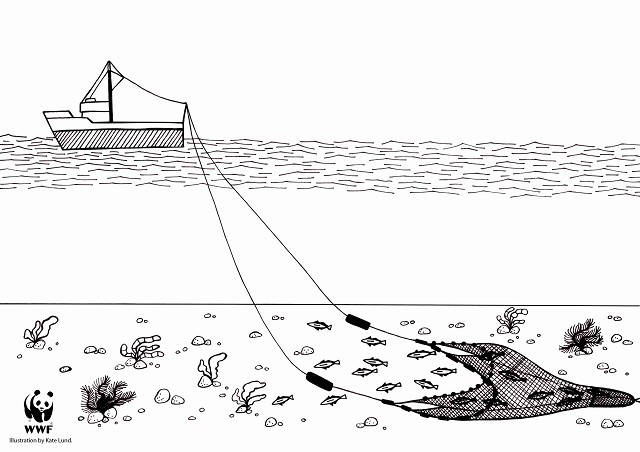
\includegraphics[width=0.65\textwidth]{DemersalTrawling.jpg} 
\end{figure}

\textbf{Intuition:} Would you expect the effect of trawl type to be additive or multiplicative?

\end{frame}


\begin{frame}[fragile]
\frametitle{Multiplicative model with categorical explanatory variable}
\framesubtitle{Trawl by-catch\ldots}
\begin{knitrout}\scriptsize
\definecolor{shadecolor}{rgb}{0.969, 0.969, 0.969}\color{fgcolor}\begin{kframe}
\begin{alltt}
\hlstd{> }\hlstd{Bycatch.df}\hlkwb{=}\hlkwd{read.table}\hlstd{(}\hlstr{"Data/Bycatch.txt"}\hlstd{,}\hlkwc{header}\hlstd{=T)}
\hlstd{> }\hlkwd{boxplot}\hlstd{(Bycatch}\hlopt{~}\hlstd{Trawl,}\hlkwc{data}\hlstd{=Bycatch.df,} \hlkwc{horizontal}\hlstd{=T,}\hlkwc{xlab}\hlstd{=}\hlstr{"Bycatch (kg)"}\hlstd{)}
\end{alltt}
\end{kframe}
\end{knitrout}



\begin{figure}
  \centering
  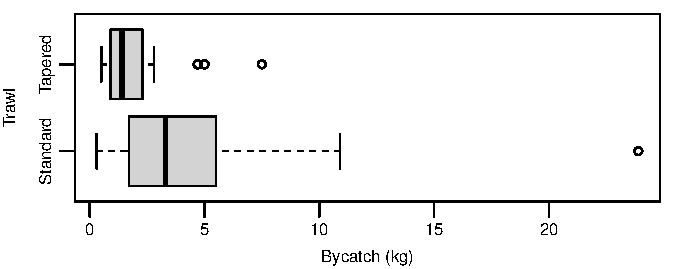
\includegraphics{figure/RC-H06-048}
\end{figure}

\begin{knitrout}\scriptsize
\definecolor{shadecolor}{rgb}{0.969, 0.969, 0.969}\color{fgcolor}\begin{kframe}
\begin{alltt}
\hlstd{> }\hlkwd{summaryStats}\hlstd{(Bycatch}\hlopt{~}\hlstd{Trawl,}\hlkwc{data}\hlstd{=Bycatch.df)}
\end{alltt}
\begin{verbatim}
         Sample Size  Mean Median  Std Dev Midspread
Standard          25 4.600    3.3 4.983138       3.8
Tapered           25 1.924    1.4 1.643999       1.4
\end{verbatim}
\end{kframe}
\end{knitrout}
\end{frame}


\begin{frame}[fragile]
\frametitle{Multiplicative model with categorical explanatory variable}
\framesubtitle{Trawl by-catch\ldots}

This seems to confirm our intuition that these data should be modelled on the log scale.
We will play stupid for now, and fit a linear model to the raw data....

\begin{knitrout}\scriptsize
\definecolor{shadecolor}{rgb}{0.969, 0.969, 0.969}\color{fgcolor}\begin{kframe}
\begin{alltt}
\hlstd{> }\hlstd{Trawl.lm}\hlkwb{=}\hlkwd{lm}\hlstd{(Bycatch}\hlopt{~}\hlstd{Trawl,}\hlkwc{data}\hlstd{=Bycatch.df)}
\hlstd{> }\hlkwd{plot}\hlstd{(Trawl.lm,}\hlkwc{which}\hlstd{=}\hlnum{1}\hlstd{)}
\end{alltt}
\end{kframe}
\end{knitrout}

% \end{frame}


% \begin{frame}[fragile]
% \frametitle{Multiplicative model with categorical explanatory variable}
% \framesubtitle{Trawl bycatch}



\begin{figure}
  \centering
  \includegraphics{figure/RC-H06-051}
\end{figure}

The \textbf{EOV} assumption is very doubtful. Normality?
\end{frame}


\begin{frame}[fragile]
\frametitle{Multiplicative model with categorical explanatory variable}
\framesubtitle{Trawl by-catch\ldots}
\begin{knitrout}\scriptsize
\definecolor{shadecolor}{rgb}{0.969, 0.969, 0.969}\color{fgcolor}\begin{kframe}
\begin{alltt}
\hlstd{> }\hlkwd{normcheck}\hlstd{(Trawl.lm)}
\end{alltt}
\end{kframe}
\end{knitrout}



\begin{figure}
  \centering
  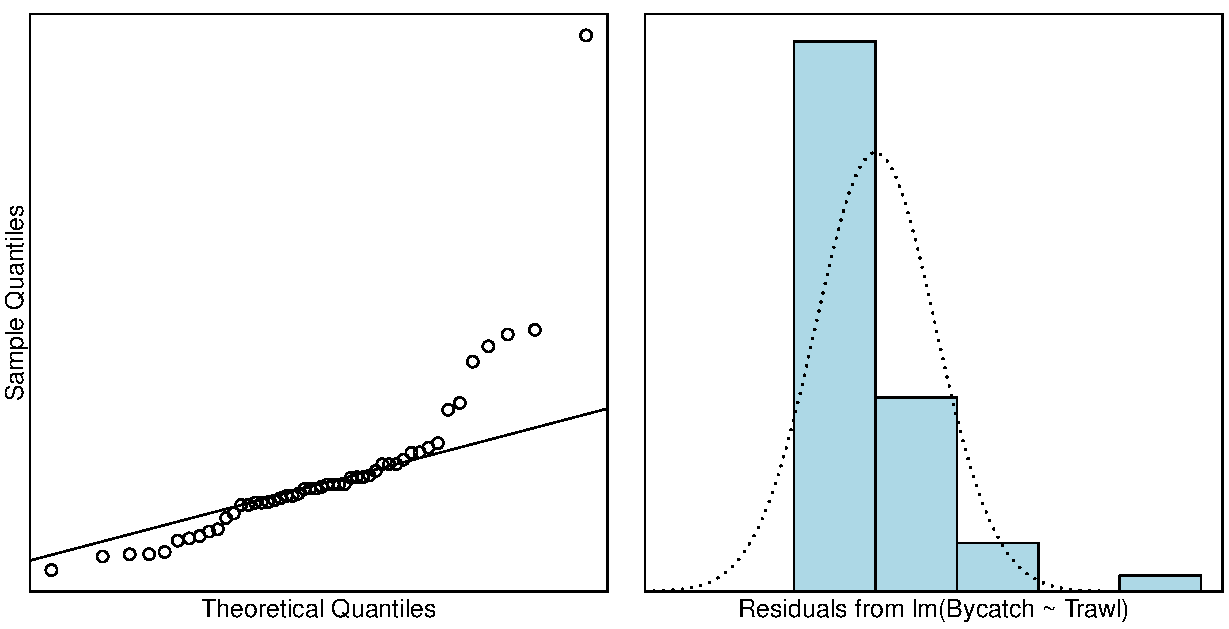
\includegraphics[scale=0.5]{figure/RC-H06-053}
\end{figure}

These plots of the residuals confirm that \textbf{EOV} and normality do not hold.
\end{frame}


\begin{frame}[fragile]
\frametitle{Multiplicative model with categorical explanatory variable}
\framesubtitle{Using logged trawl by-catch}
\begin{knitrout}\scriptsize
\definecolor{shadecolor}{rgb}{0.969, 0.969, 0.969}\color{fgcolor}\begin{kframe}
\begin{alltt}
\hlstd{> }\hlkwd{boxplot}\hlstd{(}\hlkwd{log}\hlstd{(Bycatch)}\hlopt{~}\hlstd{Trawl,}\hlkwc{data}\hlstd{=Bycatch.df,}\hlkwc{horizontal}\hlstd{=T,}\hlkwc{xlab}\hlstd{=}\hlstr{"log(Bycatch)"}\hlstd{)}
\end{alltt}
\end{kframe}
\end{knitrout}



\begin{figure}
  \centering
  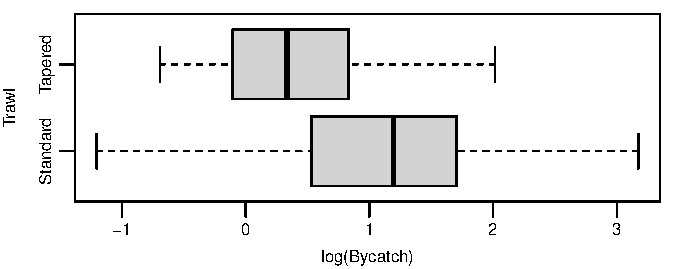
\includegraphics{figure/RC-H06-055}
\end{figure}

Looking much better. 
\end{frame}


\begin{frame}[fragile]
\frametitle{Multiplicative model with categorical explanatory variable}
\framesubtitle{Using logged trawl by-catch\ldots}

\begin{knitrout}\scriptsize
\definecolor{shadecolor}{rgb}{0.969, 0.969, 0.969}\color{fgcolor}\begin{kframe}
\begin{alltt}
\hlstd{> }\hlstd{Trawl.lmlog}\hlkwb{=}\hlkwd{lm}\hlstd{(}\hlkwd{log}\hlstd{(Bycatch)}\hlopt{~}\hlstd{Trawl,}\hlkwc{data}\hlstd{=Bycatch.df)}
\hlstd{> }\hlkwd{plot}\hlstd{(Trawl.lmlog,}\hlkwc{which}\hlstd{=}\hlnum{1}\hlstd{)}
\end{alltt}
\end{kframe}
\end{knitrout}



\begin{figure}
  \centering
  \includegraphics{figure/RC-H06-057}
\end{figure}

Sweet as.
\end{frame}


\begin{frame}[fragile]
\frametitle{Multiplicative model with categorical explanatory variable}
\framesubtitle{Using logged trawl by-catch\ldots}
\begin{knitrout}\scriptsize
\definecolor{shadecolor}{rgb}{0.969, 0.969, 0.969}\color{fgcolor}\begin{kframe}
\begin{alltt}
\hlstd{> }\hlkwd{normcheck}\hlstd{(Trawl.lmlog)}
\end{alltt}
\end{kframe}
\end{knitrout}



\begin{figure}
  \centering
  \includegraphics[scale=0.5]{figure/RC-H06-059}
\end{figure}

Looking good. 
\end{frame}


\begin{frame}[fragile]
\frametitle{Multiplicative model with categorical explanatory variable}
\framesubtitle{Using logged trawl by-catch\ldots}
\begin{knitrout}\scriptsize
\definecolor{shadecolor}{rgb}{0.969, 0.969, 0.969}\color{fgcolor}\begin{kframe}
\begin{alltt}
\hlstd{> }\hlkwd{cooks20x}\hlstd{(Trawl.lmlog)}
\end{alltt}
\end{kframe}
\end{knitrout}



\begin{figure}
  \centering
  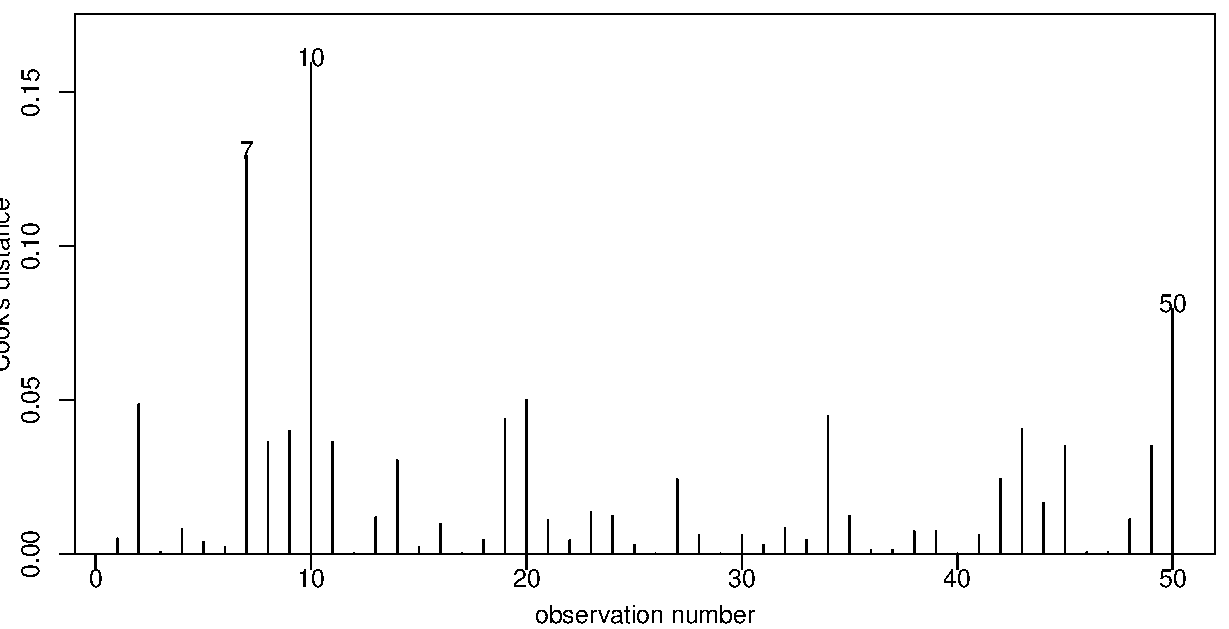
\includegraphics[scale=0.5]{figure/RC-H06-061}
\end{figure}

No problems. 
\end{frame}



\begin{frame}[fragile]
\frametitle{Multiplicative model with categorical explanatory variable}
\framesubtitle{Results: Using logged trawl by-catch}
Assumptions are satisfied. We can trust the fitted model.

\begin{knitrout}\scriptsize
\definecolor{shadecolor}{rgb}{0.969, 0.969, 0.969}\color{fgcolor}\begin{kframe}
\begin{alltt}
\hlstd{> }\hlkwd{summary}\hlstd{(Trawl.lmlog)}
\end{alltt}
\end{kframe}
\end{knitrout}

\begin{knitrout}\scriptsize
\definecolor{shadecolor}{rgb}{0.969, 0.969, 0.969}\color{fgcolor}\begin{kframe}
\begin{verbatim}
Coefficients:
             Estimate Std. Error t value Pr(>|t|)    
(Intercept)    1.0996     0.1700   6.469 4.79e-08 ***
TrawlTapered  -0.7122     0.2404  -2.963  0.00473 ** 
---
Residual standard error: 0.8498 on 48 degrees of freedom
Multiple R-squared:  0.1546,	Adjusted R-squared:  0.137 
F-statistic:  8.78 on 1 and 48 DF,  p-value: 0.004728
\end{verbatim}
\end{kframe}
\end{knitrout}
There is a statistically significance effect of trawl type (\pval{} $\approx 0.005$).

However, our model only explained 15\% of the variability in the logged data and 
will not be very good for prediction.
\end{frame}


\begin{frame}[fragile]
\frametitle{Multiplicative model with categorical explanatory variable}
\framesubtitle{Interpretation: Using logged trawl by-catch}
We need to back-transform to the raw data scale to make sense of the above results:
\medskip

\begin{knitrout}\scriptsize
\definecolor{shadecolor}{rgb}{0.969, 0.969, 0.969}\color{fgcolor}\begin{kframe}
\begin{alltt}
\hlstd{> }\hlkwd{exp}\hlstd{(}\hlkwd{confint}\hlstd{(Trawl.lmlog))}
\end{alltt}
\begin{verbatim}
                 2.5 %    97.5 %
(Intercept)  2.1336329 4.2261691
TrawlTapered 0.3025531 0.7953873
\end{verbatim}
\end{kframe}
\end{knitrout}
\medskip
The median by-catch using the tapered trawl was estimated to be between 30\% and 80\% that of the standard trawl.
\bigskip

Alternatively, 
\begin{knitrout}\scriptsize
\definecolor{shadecolor}{rgb}{0.969, 0.969, 0.969}\color{fgcolor}\begin{kframe}
\begin{alltt}
\hlstd{> }\hlnum{100}\hlopt{*}\hlstd{(}\hlkwd{exp}\hlstd{(}\hlkwd{confint}\hlstd{(Trawl.lmlog)[}\hlnum{2}\hlstd{,])}\hlopt{-}\hlnum{1}\hlstd{)}
\end{alltt}
\begin{verbatim}
    2.5 %    97.5 % 
-69.74469 -20.46127 
\end{verbatim}
\end{kframe}
\end{knitrout}
the median by-catch using the tapered trawl was estimated to be between 20\% and 70\% smaller than when using the standard trawl.
\end{frame}



%%%%%%%%%%%%%%%%%%%%%%%%%%%%%%%%%%%%%%%%%%%%%%%%%%%%%%%%%%%%%%%%%%%%%%%%%%%%%%%%%%%%%%%%%%%
\BeginSection{Closing remarks and relevant \rcode{R}-code}
%%%%%%%%%%%%%%%%%%%%%%%%%%%%%%%%%%%%%%%%%%%%%%%%%%%%%%%%%%%%%%%%%%%%%%%%%%%%%%%%%%%%%%%%%%%


\begin{frame}[fragile]
\frametitle{Closing remarks}
\textbf{NOTE:} Any of the types of linear model that you encounter {\em could} be
applied to logged data if that is more appropriate, either due to rationale and/or 
due to right-skewness in the data.\\
\bigskip
In all cases you will follow the same procedure:\\
\bigskip
\begin{enumerate}[1.]\setlength{\itemsep}{5mm}
\item Fit the linear model to the logged data.
\item Back-transform (i.e., exponentiate) the relevant estimated coefficients, and confidence or 
prediction intervals.
\item \textbf{Remember} that the effect is multiplicative, 
and that back-transformed coefficients and CIs are for the median.
\end{enumerate}
\end{frame}



\begin{frame}[fragile]

\frametitle{Most of the new \rcode{R}-code you need for this chapter}
If any of the following hold:
\begin{itemize}
\item A multiplicative effect of the explanatory variables seems appropriate
\item Right skewness of the variability (inspect the residuals to check)
\item A funnel effect in the plot of residuals vs fitted values
\end{itemize}
then a log transformation of the response variable $y$ may be appropriate. The usual steps (fitting a linear model and assumption checking, CIs, etc) are then applied to the logged response.


\begin{knitrout}\scriptsize
\definecolor{shadecolor}{rgb}{0.969, 0.969, 0.969}\color{fgcolor}\begin{kframe}
\begin{alltt}
\hlstd{> }\hlstd{Trawl.lmlog}\hlkwb{=}\hlkwd{lm}\hlstd{(}\hlkwd{log}\hlstd{(Bycatch)}\hlopt{~}\hlstd{Trawl,}\hlkwc{data}\hlstd{=Bycatch.df)}
\hlstd{> }\hlcom{# then check if it's okay}
\hlstd{> }\hlkwd{plot}\hlstd{(Trawl.lmlog,}\hlkwc{which}\hlstd{=}\hlnum{1}\hlstd{)}
\end{alltt}
\end{kframe}
\end{knitrout}


Confidence intervals can be back-transformed and interpreted as a multiplicative increases/decreases - in this case relative to baseline:


\begin{knitrout}\scriptsize
\definecolor{shadecolor}{rgb}{0.969, 0.969, 0.969}\color{fgcolor}\begin{kframe}
\begin{alltt}
\hlstd{> }\hlkwd{exp}\hlstd{(}\hlkwd{confint}\hlstd{(Trawl.lmlog))}
\end{alltt}
\begin{verbatim}
                 2.5 %    97.5 %
(Intercept)  2.1336329 4.2261691
TrawlTapered 0.3025531 0.7953873
\end{verbatim}
\end{kframe}
\end{knitrout}

and we interpret this with respect to change in the median value of $y$.

\end{frame}

\end{document}

